% !TEX encoding = UTF-8 Unicode
\documentclass[10pt,usepdftitle=false,aspectratio=169]{beamer}
\usepackage[left]{muibkitsec}
\usepackage{listings}

\usepackage{microtype}
\usepackage{graphbox}
\usepackage{booktabs} 

\usepackage{amsmath,amssymb,amsfonts,amsthm,mathtools}
\usepackage{algorithmic}
\usepackage{textcomp}
\usepackage{xcolor}
\usepackage{diagbox}
\usepackage{float, multirow}
\usepackage{tikz, pgfplots}
\usepackage{tikzsymbols}
\usetikzlibrary{spy}
\usepackage{subcaption}
\usepgfplotslibrary{groupplots}
\pgfplotsset{compat=newest}

% ------------------------------------------------------------------------
\title{Adversarial Label Flips}
\subtitle{Related work presentation}
\author{Matthias Dellago \& Maximilian Samsinger}
\date{22 January 2021}

% ------------------------------------------------------------------------

\begin{document}
\DeclarePairedDelimiter\abs{\lvert}{\rvert}%
\DeclarePairedDelimiter\norm{\lVert}{\rVert}%
\DeclarePairedDelimiter\ceil{\lceil}{\rceil}
\DeclarePairedDelimiter\floor{\lfloor}{\rfloor}

\begin{frame}[plain]
	\maketitle
\end{frame}	

%1x Introduction
%1x Slide Angriffe
%1x Slide Pytorch
%1x Slide Foolbox 
%1x Slide Datensätze
%1x Slide Pytorch
%
%
%1x Slide Architectures

%\begin{frame}[fragile]
%	\frametitle{Introduction/Reminder from last time}
%	\begin{columns}
%		\begin{column}{.5\columnwidth}
%			\begin{block}{Adversarial examples}
%				Generate adversarial examples. Create confusion matrix
%			\end{block}
%		\end{column}
%		\begin{column}{.5\columnwidth}
%			\begin{exampleblock}{Confusion matrix}
%				Confusion matrix from last presentation
%			\end{exampleblock}
%		\end{column}
%	\end{columns}
%\end{frame}

\begin{frame}[fragile]
	\frametitle{Standard sources on adversarial examples}
	\begin{columns}
		\begin{column}{.5\columnwidth}
			\begin{block}{Adversarial examples \cite{Szegedy13}}
				Deep neural networks are vulnerable to adversarial perturbations!
			\end{block}
			\only<2-3>{\begin{alertblock}{Fast gradient sign method \cite{goodfellow2014explaining}}
					Even worse: Adversarial examples generalize over multiple datasets and architectures. Even cheap attacks like FGSM can work.
					\end{alertblock}}
			\only<4->{\begin{alertblock}{Projected gradient descent \cite{madry2017towards}}
					Strong and cheap attacks therefore exist: Projected gradient descent (PGD) iteratively computes FGSM. 
				\end{alertblock}}
		\end{column}
	\visible<3->{
		\begin{column}{.5\columnwidth}
			\begin{alertblock}{Fast gradient sign method}
				Modify an input image $x$, with respective label $y$,
				\[x + \epsilon\operatorname{sign}(\nabla_x\ J(\theta,x,y)). \] 
				using the loss function $J$. 
			\end{alertblock}
		\end{column}}
	\end{columns}
	\only<1-3>{\source{[1] Intriguing properties of neural networks, 2013\\ {[2]} Explaining and harnessing adversarial examples, 2014}}
	\only<4->{\source{[1] Intriguing properties of neural networks, 2014\\ {[3]} Towards deep learning models resistant to adversarial attacks, 2018}}

\end{frame}

\begin{frame}[noframenumbering,fragile]
	\frametitle{Fast gradient sign method}
	\begin{tabular}{ccccc}
		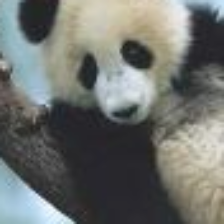
\includegraphics[align=c,width=0.28\columnwidth]{plots/panda_577.png} & \Huge{+} & \Huge{\textbf{$\epsilon$}}\ 
\includegraphics[align=c,width=0.28\columnwidth]{plots/nematode_082.png}\ & \Huge{=} & 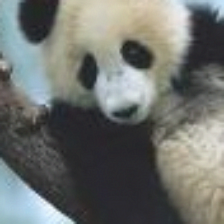
\includegraphics[align=c,width=0.28\columnwidth]{plots/gibbon_993.png} \\~\\
		\huge{Panda} &&\qquad \large{$\operatorname{sign}(\nabla_x\ J(\theta,x,y))$}&& \huge{Gibbon} \\
		(57.7\% confidence) &&&& (99.3\% confidence) 
	\end{tabular}
	\source{[2] Explaining and harnessing adversarial examples, 2014}
\end{frame}

\begin{frame}[fragile]
	\frametitle{What we want to do}
	\begin{block}{Confusion Matrix}
		\begin{table}
			\setlength{\extrarowheight}{2pt}
			\begin{tabular}{cc|c|c|c|}
				& \multicolumn{1}{c}{} & \multicolumn{3}{c}{Categorised as}\\
				& \multicolumn{1}{c}{} & \multicolumn{1}{c}{Dog}  & \multicolumn{1}{c}{Cat} & \multicolumn{1}{c}{Plane} \\\cline{3-5}
				\multirow{3}*{Adversarial Example of a}  & Dog & 0.0 & ? & ?\\\cline{3-5}
				& Cat & ? & 0.0 &  ? \\\cline{3-5}
				& Plane & ? & ? &  0.0 \\\cline{3-5}
			\end{tabular}
		\end{table}
		How many modified dogs get classified as cats vs as planes? etc.
	\end{block}
\end{frame}

\begin{frame}[fragile]
	\frametitle{Case study}
	
\end{frame}

\begin{frame}[fragile]
	\frametitle{Foolbox}
	A suit of attacks is available with FoolBox! \cite{rauber2017foolbox}
	\visible<2>{\begin{block}{Foolbox}
			\begin{itemize}
				\item Over 40 different attacks.
				\item Available in PyTorch, TensorFlow and JAX.
				\item Easy to work with.
			\end{itemize}
	\end{block}}
	\source{[4] Foolbox: A python toolbox to benchmark the robustness of machine learning models, 2017}
\end{frame}

\begin{frame}[fragile]
	\frametitle{Foolbox}
	Projected Gradient Descent (PGD) attack for different \texttt{epsilons}.
	\visible<2->{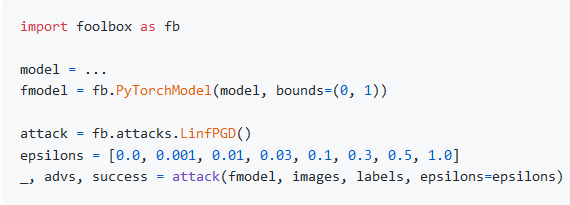
\includegraphics[scale=0.9]{plots/minimal_example_foolbox.png}}
	\source{[4] Foolbox: A python toolbox to benchmark the robustness of machine learning models, 2017}
\end{frame}

\begin{frame}[fragile]
	\frametitle{Datasets}
\end{frame}

\begin{frame}[fragile]
	\frametitle{MNIST \cite{deng2012mnist}}
	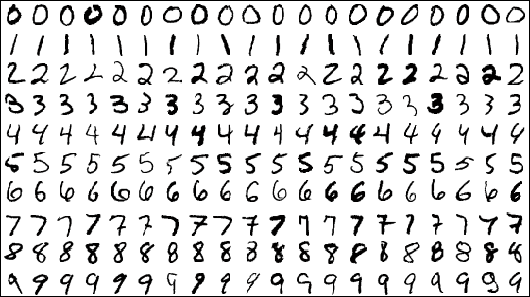
\includegraphics[width=\linewidth]{plots/MNIST.png}
	\source{The MNIST database of handwritten digit images for machine learning research, 2012}
\end{frame}

\begin{frame}[fragile]
	\frametitle{Fashion-MNIST \cite{xiao2017fashion}}
	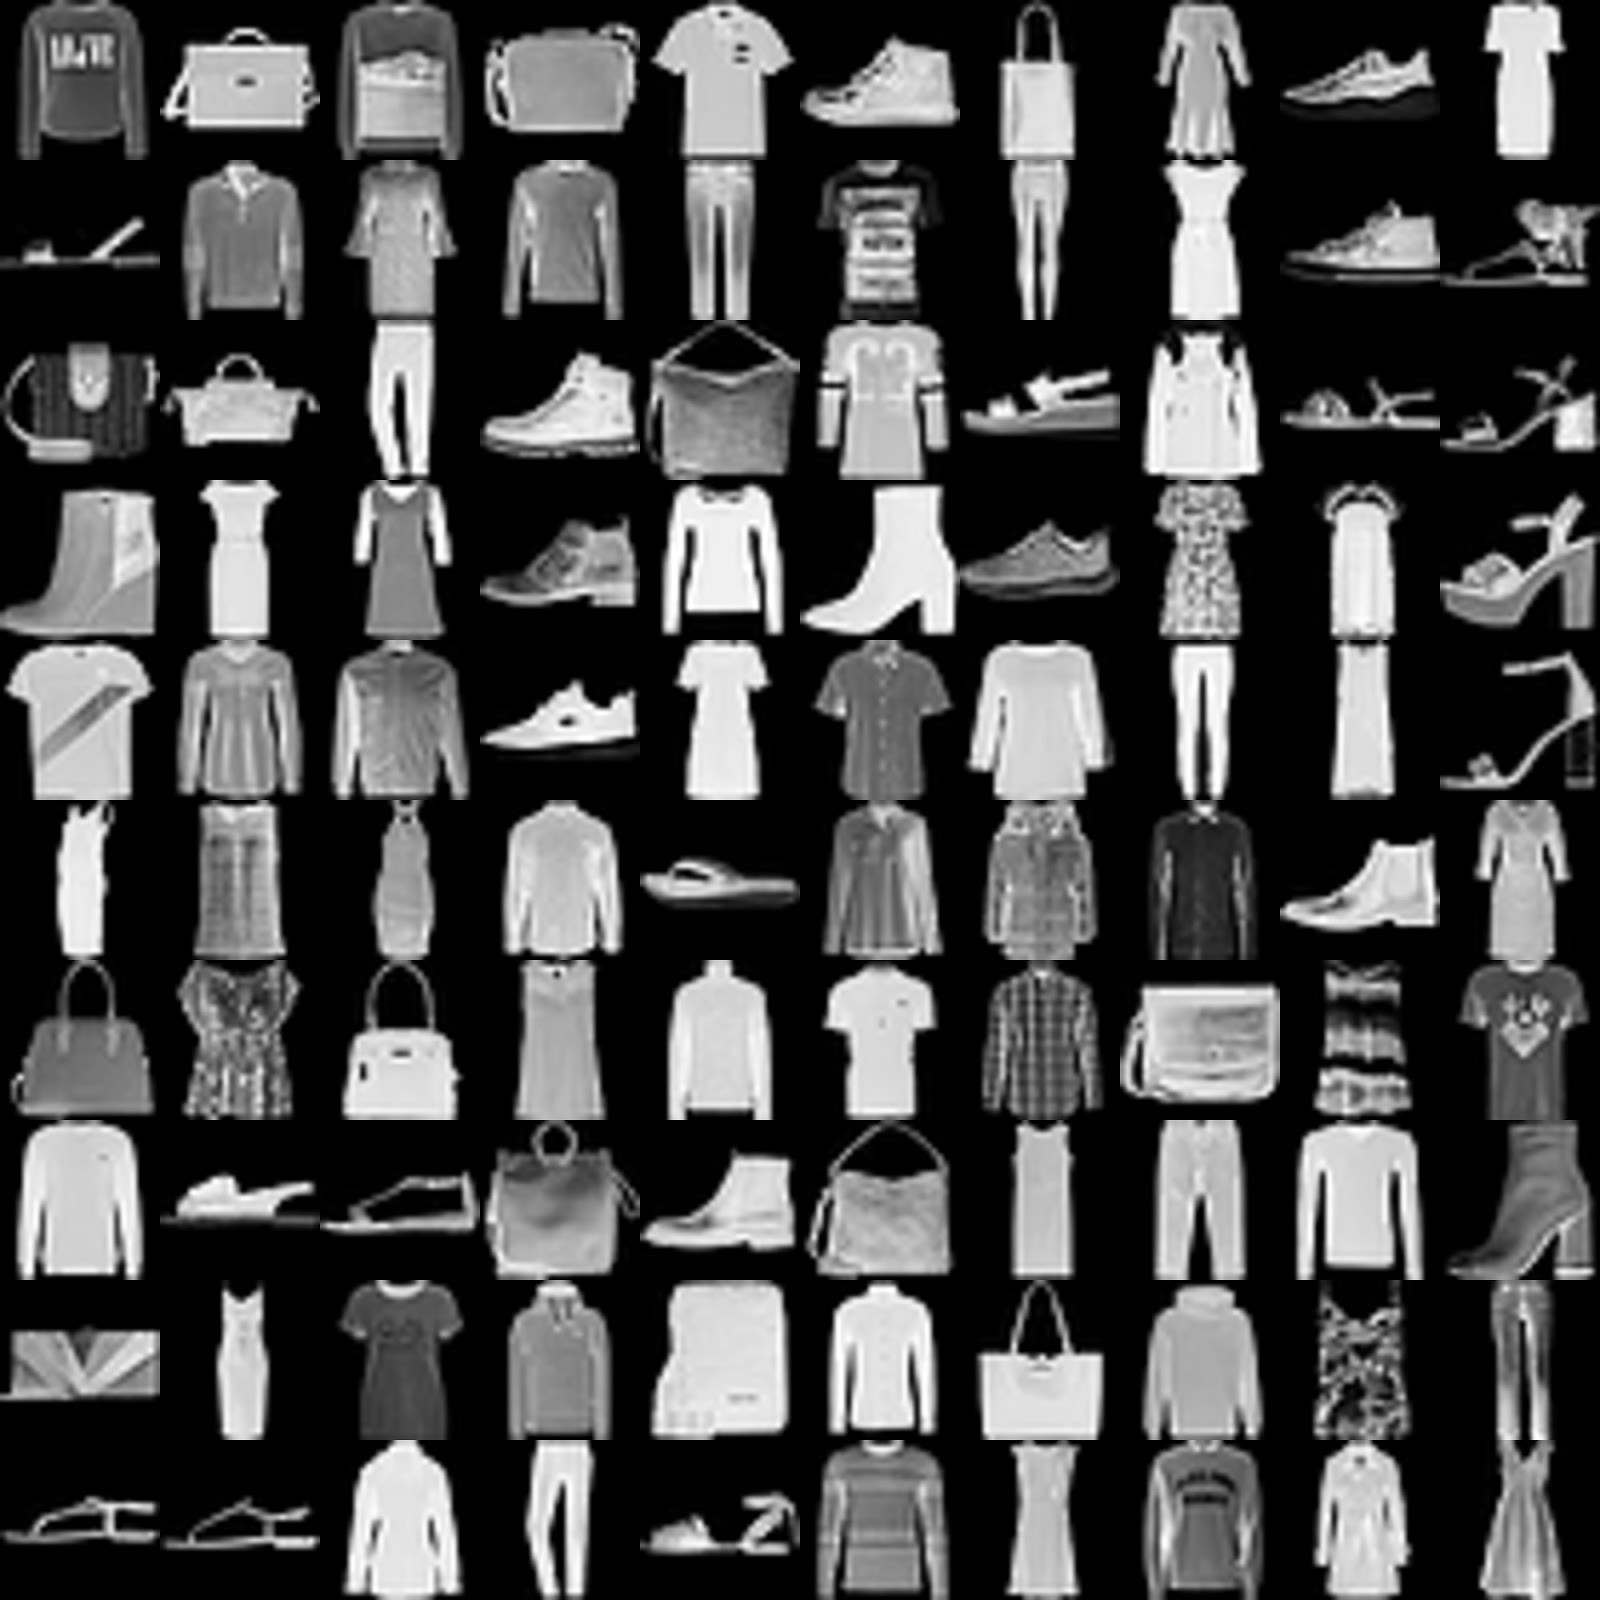
\includegraphics[scale=0.105]{plots/Fashion-MNIST.jpg}
	\source{Fashion-MNIST: A novel image dataset for benchmarking machine learning algorithms, 2017}
\end{frame}

\begin{frame}[fragile]
	\frametitle{CIFAR-10 \cite{krizhevsky2009learning}}
	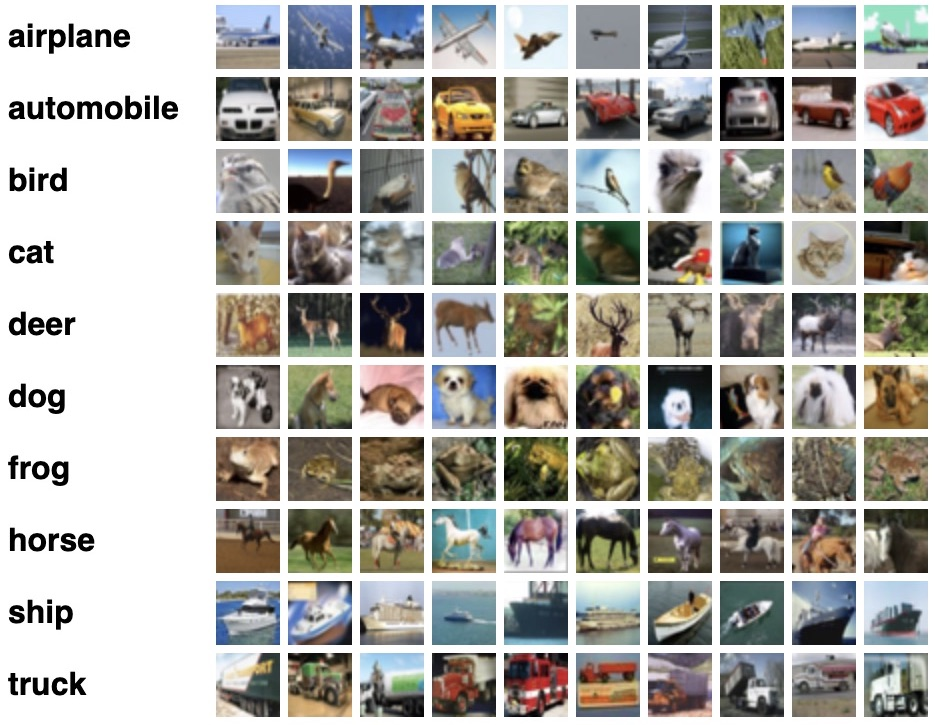
\includegraphics[scale=0.23]{plots/CIFAR-10.jpg}
	\source{Learning multiple layers of features from tiny images, 2009}
\end{frame}


%\begin{frame}[fragile]
%	\frametitle{Optional Slide 2: Convolutional neural networks}
%	We use small convolutional neural networks \cite{lecun1999object} for the "easy" data sets. For CIFAR-10 we will use ResNet-18, a residual neural network \cite{he2016deep}, \cite{he2016identity}.
%\end{frame}

\begin{frame}[allowframebreaks]
	\frametitle{References}
	\bibliographystyle{unsrt}
	\bibliography{literature}
\end{frame}


\end{document}
